% ============================================================================
% Experiments — DUET
% ============================================================================

\section{Experiments}
\label{sec:experiments}

\subsection{Setup}
\label{sec:setup_exp}

\paragraph{Environments.}
We evaluate DUET on two interactive LLM-agent benchmarks through the AgentGym-based evaluation toolkit~\citep{xi2024agentgym}.
\textbf{ALFWorld}~\citep{shridhar2020alfworld} is a text-based household instruction-following environment with long action horizons and sparse goal-completion rewards.
\textbf{WebShop}~\citep{yao2022webshop} is a simulated e-commerce navigation environment with structured product search, attribute matching, and partial-credit rewards.
For both environments, we report test-set success rate using the same evaluation protocol for all methods.

\paragraph{Models.}
We use Qwen2.5-1.5B-Instruct and Qwen2.5-3B-Instruct as student policies where teach-replay is highly beneficial.
The teacher data is a fixed offline trajectory cache collected from Qwen2.5-72B-Instruct and filtered to successful executions.
The same teacher cache is used for all methods that require teacher trajectories.

\paragraph{Baselines.}
We compare against four baselines:
(i) \textbf{OnPolicy GRPO}~\citep{shao2024deepseekmath}, which uses no teacher data;
(ii) \textbf{LUFFY}~\citep{yan2025luffy}, which mixes teacher trajectories into GRPO with a policy-shaping term;
(iii) \textbf{CHORD}~\citep{zhang2025chord}, which adds a manually scheduled supervised objective on top of teacher-mixed GRPO; and
(iv) \textbf{SFT$+$GRPO}, which first trains on teacher data with supervised learning and then continues with on-policy GRPO.
Implementations of LUFFY and CHORD follow the authors' released code where available.

\paragraph{Training protocol.}
All methods use the same GRPO backbone, batch size, group size, optimizer, KL coefficient, teacher cache, and total training budget.
We train each method for 100 update steps, using a fixed training budget rather than tuning the horizon separately for each method.
For teacher-replay methods, each group contains both on-policy student rollouts and replayed teacher trajectories under the same mixing ratio.
Additional implementation details are provided in Appendix~\ref{app:impl}.

\subsection{Main results}
\label{sec:main_results}

Table~\ref{tab:main_results} reports test-set success rate after the fixed 100-step training budget.
DUET achieves the highest success rate among all reproduced baselines in all four model--environment settings, improving over the strongest non-DUET baseline by an average of 13.0 percentage points.

\begin{table}[t]
\centering
\caption{
\textbf{Main results.}
Test-set success rate on ALFWorld and WebShop under a fixed 100-step training budget.
Best result in each column is shown in bold; the strongest non-DUET baseline is underlined.
The $\Delta$ row reports DUET's gain over the strongest non-DUET baseline.
}
\label{tab:main_results}
\resizebox{\linewidth}{!}{
\begin{tabular}{lcccc}
\toprule
Method & 1.5B-ALFWorld & 1.5B-WebShop & 3B-ALFWorld & 3B-WebShop \\
\midrule
OnPolicy GRPO & 1.0\% & 0.5\% & 47.0\% & 2.0\% \\
LUFFY & 5.5\% & 5.5\% & 61.5\% & 38.0\% \\
CHORD & 27.0\% & 11.5\% & 67.0\% & 39.0\% \\
SFT$+$GRPO & \underline{30.0\%} & \underline{18.5\%} & 59.5\% & 24.0\% \\
DUET (Ours) & \textbf{47.5\%} & \textbf{36.0\%} & \textbf{77.5\%} & \textbf{45.5\%} \\
\midrule
$\Delta$ vs. strongest baseline & +17.5pp & +17.5pp & +10.5pp & +6.5pp \\
\bottomrule
\end{tabular}
}
\end{table}

\paragraph{DUET helps most in the cold-start regime.}
The gains are largest for the weaker 1.5B students, where on-policy GRPO receives little useful reward signal.
On 1.5B, DUET improves over the strongest baseline by 17.5 percentage points on both ALFWorld and WebShop.
The gains remain positive for the 3B students, but the margins are smaller, consistent with stronger students suffering less from cold start.

\paragraph{Teacher mixing alone is not enough.}
LUFFY improves over purely on-policy GRPO in most settings, confirming that teacher trajectories are useful.
However, directly mixing teacher data does not address baseline contamination or off-policy mismatch.
CHORD obtains stronger cold-start performance by adding supervised learning on teacher trajectories, but its teacher influence is controlled by a predefined schedule.
DUET improves over these baselines by combining corrected teacher-action replay with progress-based reward shaping from teacher states.

\paragraph{Gain magnitude follows the cold-start pattern.}
Equation~\eqref{eq:baseline_contamination} suggests that baseline contamination is strongest when the on-policy success rate $p_o$ is small.
The empirical pattern is consistent with this prediction: DUET's gain over the strongest non-DUET baseline is +17.5pp on both 1.5B settings, where on-policy GRPO nearly collapses, and decreases to +10.5pp / +6.5pp on the 3B settings, where the on-policy stream already provides useful signal.
This pattern supports the view that DUET is most valuable when teacher replay is needed but direct teacher mixing is most biased.

\paragraph{Learning dynamics.}
Figure~\ref{fig:learning_curves} shows training curves under the fixed 100-step budget.
DUET attains the strongest final performance in all four panels and also shows more stable improvements, with the clearest separation in the 1.5B settings.
On ALFWorld, the curves report on-policy success rate.
On WebShop, they report mean reward to reflect the environment's partial-credit feedback during training.

\begin{figure}[t]
\centering
\IfFileExists{figures/fig_learning_curves.pdf}{%
  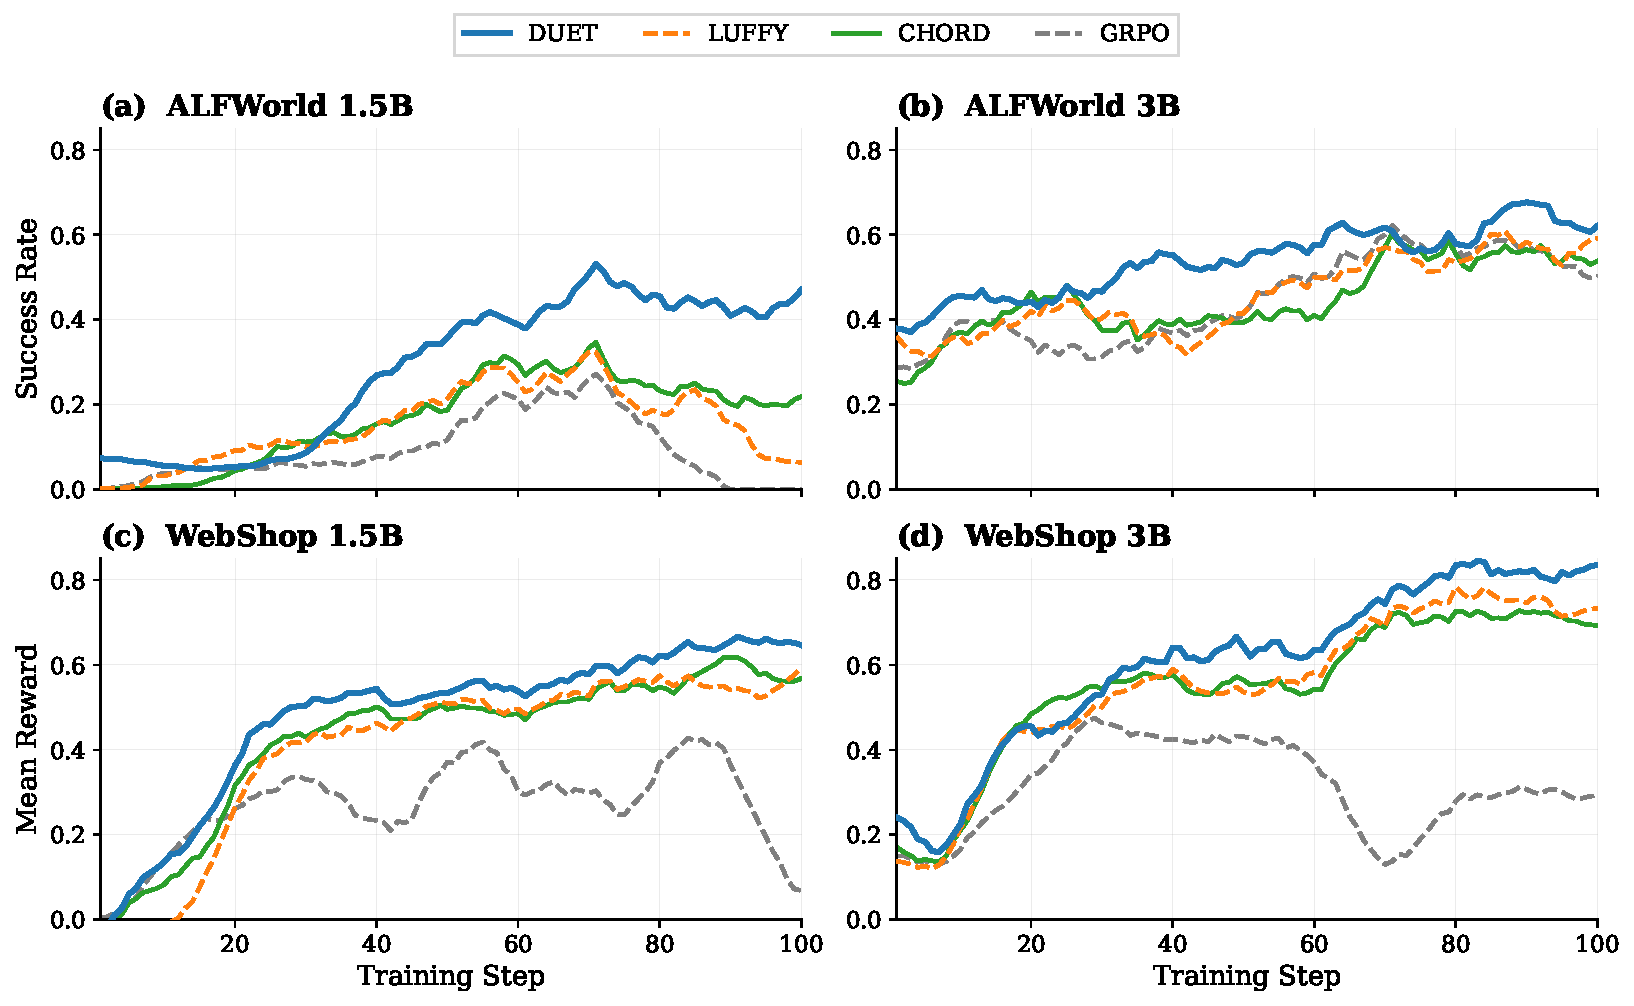
\includegraphics[width=0.99\linewidth]{figures/fig_learning_curves.pdf}%
}{%
  
\includegraphics[width=0.99\linewidth]{fig_learning_curves.pdf}%
}
\caption{
\textbf{Learning curves under the fixed 100-step budget.}
The y-axis reports on-policy success rate on ALFWorld and mean reward on WebShop.
DUET improves final performance in all four model--environment settings, with the clearest gains in the 1.5B cold-start regime.
}
\label{fig:learning_curves}
\end{figure}

\subsection{Component ablations}
\label{sec:ablations}

Table~\ref{tab:ablation} ablates DUET's components on the 1.5B settings, where cold start makes the differences most visible.
Each row removes one component while keeping the rest of the configuration fixed.

\begin{table}[t]
\centering
\caption{
\textbf{Component ablations on 1.5B students.}
Each row removes one DUET component while keeping all others fixed.
The rightmost column reports the average drop from full DUET across the two environments.
}
\label{tab:ablation}
\resizebox{0.92\linewidth}{!}{
\begin{tabular}{llccc}
\toprule
Variant & Component removed & 1.5B-AF & 1.5B-WS & Avg. $\Delta$ \\
\midrule
DUET (full) & -- & 47.5\% & 36.0\% & -- \\
w/o baseline sep. & Advantage normalization & 0.0\%$^\star$ & 0.0\%$^\star$ & $-41.8$pp \\
w/o DR3 weighting & Density-ratio correction & 38.5\% & 9.5\% & $-17.8$pp \\
w/o State Channel & Progress reward shaping & 31.0\% & 1.0\% & $-25.8$pp \\
w/o BC & Cold-start imitation & 34.0\% & 16.5\% & $-16.5$pp \\
\midrule
OnPolicy GRPO & No teacher data & 1.0\% & 0.5\% & -- \\
\bottomrule
\end{tabular}
}
\vspace{0.3em}
\begin{flushleft}
{\footnotesize $^\star$ Training collapses to 0\% within the first $\sim$50 steps when baseline separation is removed.}
\end{flushleft}
\end{table}

\paragraph{Baseline separation is critical.}
Removing baseline separation collapses both 1.5B settings to 0.0\%, making it the largest ablation effect.
This matches the failure mode predicted by Eq.~\eqref{eq:baseline_contamination}: without separation, high-reward teacher trajectories shift the baseline upward and suppress credit for rare successful on-policy rollouts.

\paragraph{Visualizing the contamination bias.}
Figure~\ref{fig:advantage_distribution} shows per-trajectory advantage distributions on 1.5B-ALFWorld at three training stages, with and without baseline separation.
With baseline separation, the on-policy mean stays near zero throughout training ($\mu_{\rm on}=0.06,0.05,0.04$).
Without it, the on-policy distribution drifts negative as teacher rewards raise the shared baseline ($\mu_{\rm on}=0.02\rightarrow -0.04\rightarrow -0.17$).
This matches the sign and direction predicted by Eq.~\eqref{eq:baseline_contamination}, and provides a direct visual explanation for the collapse observed in Table~\ref{tab:ablation}.

\begin{figure}[t]
\centering
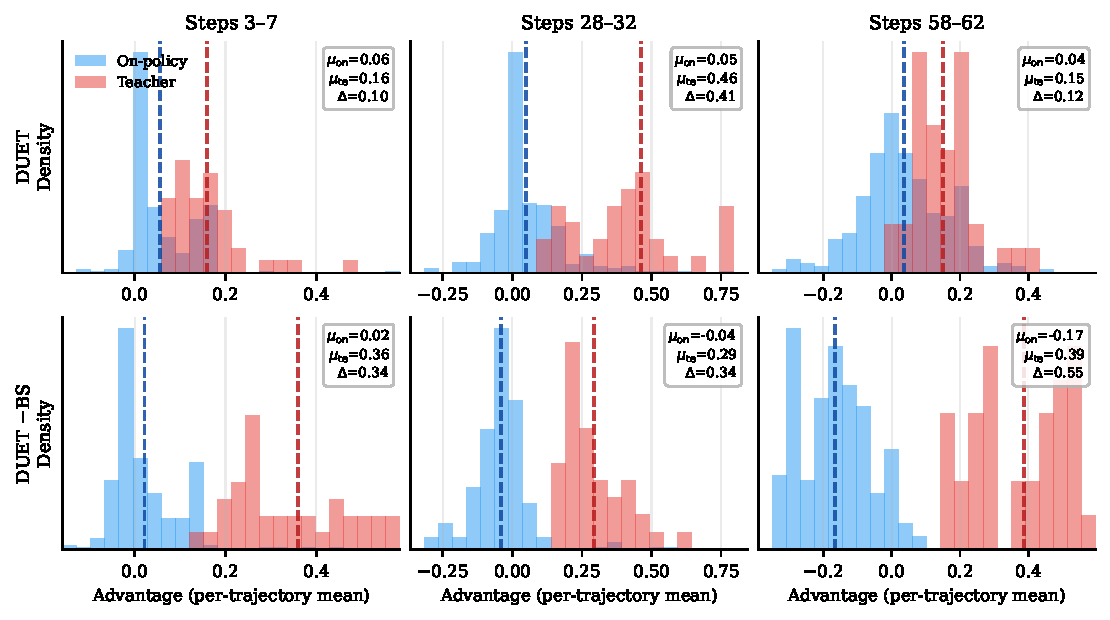
\includegraphics[width=0.86\linewidth]{figures/fig_advantage_dist.pdf}
\caption{
\textbf{Advantage distributions with and without baseline separation} on 1.5B-ALFWorld.
Top row: full DUET; on-policy means stay near zero throughout training.
Bottom row: DUET with baseline separation removed; on-policy means drift negative as teacher rewards inflate the shared GRPO baseline, in the direction predicted by Eq.~\eqref{eq:baseline_contamination}.
}
\label{fig:advantage_distribution}
\end{figure}

\paragraph{Different components address different failure modes.}
Removing the State Channel reduces performance by 16.5pp on ALFWorld and 35.0pp on WebShop, showing that progress-based shaping provides substantial exploration guidance.
Removing DR3 causes a significant drop on both environments, suggesting that distribution correction matters most when the teacher--student gap persists over longer or more diverse interactions.
Behavior cloning also contributes in both environments by providing dense cold-start supervision before the discriminator-based correction stabilizes.

\subsection{Action Channel dynamics}
\label{sec:dynamics}

The Action Channel is designed to reduce teacher influence according to training signals rather than a fixed step schedule.
Figure~\ref{fig:dynamics} reports the quantities that control this behavior.
The effective teacher replay weight decreases over training, the BC coefficient decays from its cold-start value, and discriminator accuracy rises above chance.
Together, these trends indicate that DUET relies most strongly on teacher actions early in training and gradually attenuates their effect.

\begin{figure}[t]
\centering
\IfFileExists{figures/fig3_self_attenuation.pdf}{%
  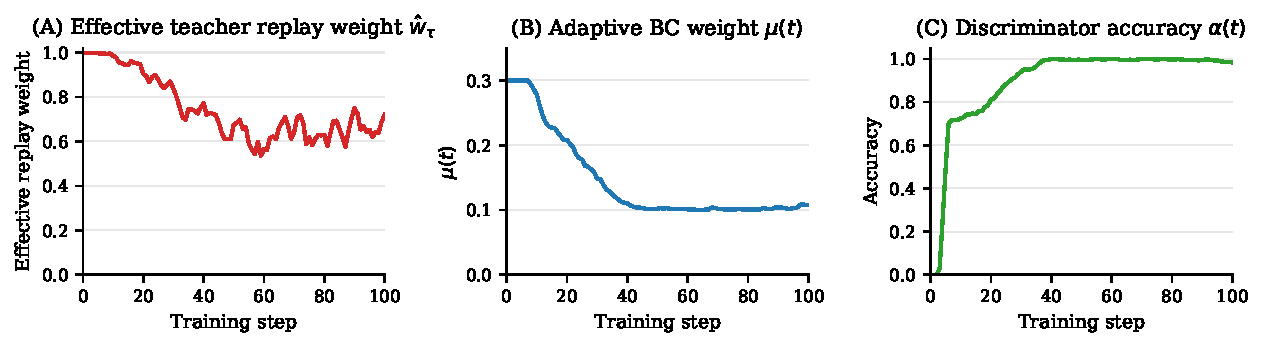
\includegraphics[width=0.86\linewidth]{figures/fig3_self_attenuation.pdf}%
}{%
  
\includegraphics[width=0.86\linewidth]{fig3_self_attenuation.pdf}%
}
\caption{
\textbf{Self-attenuation in the Action Channel.}
(A) The effective teacher replay weight $\hat{w}_\tau$ decreases over training.
(B) The adaptive behavior-cloning coefficient $\mu(t)$ decays after the cold-start phase.
(C) Discriminator accuracy $\alpha(t)$ rises above chance, providing the signal used to attenuate teacher-action influence.
}
\label{fig:dynamics}
\end{figure}

\paragraph{Two complementary fade-out paths.}
DUET reduces teacher influence through two signals.
The first comes from asymmetric baseline separation: by Eq.~\eqref{eq:teacher_advantage}, the teacher centered reward is proportional to $(1-p_o)$, so it shrinks as on-policy success improves.
The second comes from DR3: $\hat w$ tracks the teacher--student distribution gap and decreases as teacher samples become easier to distinguish from on-policy samples.
These mechanisms respond to reward progress and distributional progress, respectively, allowing teacher influence to recede without a fixed step-indexed schedule.